
\de{ĐỀ THI GIỮA HỌC KỲ I NĂM HỌC 2022-2023}{THPT Bình Chiểu - Đề 123}

\begin{bt}%[Dự án đề kiểm tra GHKI NH22-23- Nguyễn Sĩ Đạt]%[0T1Y3-1]%Câu 1:
Cho $A=\{0; 2; 3; 5; 6\}$; $B=\{1; 2; 3; 4; 5\}$. Tìm $A \cap B$, $A \cup B$.
\loigiai{
	Ta có $A\cap B=\{2;3;5\}$ và $A\cup B=\{0;1;2;3;4;5;6\}$.
}
\end{bt}
\begin{bt}%[Dự án đề kiểm tra GHKI NH22-23- Nguyễn Sĩ Đạt]%[0T1B3-2]%Câu 2:
Cho $A=(-\infty ; 7]$; $B=[2; 10]$. Tìm $A \cap B$, $A \cup B$, $C_{\mathbb{R}} A$.
\loigiai{
	Ta có  $A\cap B=[2;7]$, $A\cup B=(-\infty;10]$ và $\mathrm{C}_{\mathbb{R}}A=(7; +\infty)$. 
}
\end{bt}
\begin{bt}%[Dự án đề kiểm tra GHKI NH22-23- Nguyễn Sĩ Đạt]%[0T2B1-2]%Câu 3:
Biểu diễn miền nghiệm của bất phương trình sau trên mặt phẳng tọa độ: $x+4 y \geq 8$.
\loigiai{
	\immini{
		Đường thẳng $\Delta\colon x+4y=8$ đi qua hai điểm $A(0;2)$ và $B(8;0)$.\\
		Kết luận: Miền nghiệm của bất phương trình là phần không gạch chéo, tính cả đường thẳng $\Delta$.
	}{
		\begin{tikzpicture}[scale=0.4, line join=round, line cap=round, >=stealth]
			\tikzset{every node/.style={scale=0.8}}
			\def\xmin{-1}\def\xmax{9.5}\def\ymin{-1}\def\ymax{3}
			\fill [pattern=north east lines,pattern color=blue!20] plot[smooth,samples=200,domain=\xmin:\xmax](\x,{-1/4*(\x)+2})--
			(\xmax,\ymin)--(\xmin,\ymin);
			\draw (0,2)--(8,0)node[pos=0.5,above,sloped]{$\Delta\colon x+4y=8$};
			\draw[->] (\xmin-0.2,0)--(\xmax+0.3,0) node[above] {$x$};
			\draw[->] (0,\ymin-0.2)--(0,\ymax+0.3) node[left] {$y$};
			\draw (0,0) node [below left] {$O$};
			\foreach \x in {8}\draw (\x,0.1)--(\x,-0.1) node [above] {$\x$};
			\foreach \y in {2}\draw (0.1,\y)--(-0.1,\y) node [above right] {$\y$};
			\clip (\xmin,\ymin) rectangle (\xmax,\ymax);
			\draw[thick,smooth,samples=200,domain=\xmin:\xmax] plot (\x,{-1/4*(\x)+2});
		\end{tikzpicture}
	}
}
\end{bt}
\begin{bt}%[Dự án đề kiểm tra GHKI NH22-23- Nguyễn Sĩ Đạt]%[0T2K2-2]%Câu 4:
Một học sinh trường THPT Bình Chiểu dự định gấp hạc và làm hoa để đem bán gây quỹ từ thiện giúp đỡ một học sinh trong trường mắc bệnh hiểm nghèo. Cần 3 phút để gấp 1 con hạc và 5 phút để làm được bông hoa. Biết 1 con hạc bán giá $2.000$ đồng, 1 bông hoa bán giá $3.000$ đồng và học sinh này có không qu 60 phút để làm. Tổng số sản phẩm không vượt quá 16. Hỏi bạn cần làm bao nhiêu sản phẩm mỗi loại để thu được nhiều tiền nhất?
\loigiai{
	\immini{
		Gọi $x$, $y$ $(x,y\ge0)$ lần lượt là số con hạc và số bông hoa.\\
		Số tiền thu được sau khi bán: $F(x,y)=2x+3y$ (nghìn đồng).\\
		Theo đề bài, ta có hệ bất phương trình: $\heva{&3x+5y\le60\\&x+y\le16\\&x\ge0\\&y\ge0.}$\\
		Miền nghiệm của hệ là miền tứ giác $OABC$, kể cả biên với các đỉnh lần lượt là $O(0;0)$, $A(0;12)$, $B(10;6)$, $C(16;0)$.
	}{
		\begin{tikzpicture}[scale=0.27, line join=round, line cap=round, >=stealth]
			\tikzset{every node/.style={scale=1}}
			\def\xmin{-2}\def\xmax{22}\def\ymin{-2}\def\ymax{18}
			\draw[->] (\xmin-0.2,0)--(\xmax+0.2,0) node[below] {$x$};
			\draw[->] (0,\ymin-0.2)--(0,\ymax+0.2) node[right] {$y$};
			\clip (\xmin,\ymin) rectangle (\xmax,\ymax);
			\fill [pattern=north east lines,pattern color=gray] (\xmin,0)--(\xmax,0)--
			(\xmax,\ymin)--(\xmin,\ymin);
			\fill [pattern=north east lines,pattern color=gray] (0,\ymin)--(0,\ymax)--(\xmin,\ymax)--(\xmin,\ymin);
			\fill [pattern=north east lines,pattern color=red!20] plot[samples=20,domain=\xmin:\xmax] (\x,{-1*(\x)+16})--(\xmax,\ymin)--(\xmax,\ymax)--(\xmin,\ymax);
			\fill [pattern=north east lines,pattern color=blue!20] plot[samples=20,domain=\xmin:\xmax] (\x,{-3/5*(\x)+12})--(\xmax,\ymin)--(\xmax,\ymax)--(\xmin,\ymax);
			\draw (0,0) node [above right] {$O$};
			\foreach \x in {10,16,20}\draw (\x,0.1)--(\x,-0.1) node [below] {$\x$};
			\foreach \y in {6,12,16}\draw (0.1,\y)--(-0.1,\y) node [left] {$\y$};
			\clip (\xmin,\ymin) rectangle (\xmax,\ymax);
			\draw[thick,smooth,samples=200,domain=\xmin:\xmax] plot (\x,{-1*(\x)+16});
			\draw[thick,smooth,samples=200,domain=\xmin:\xmax] plot (\x,{-3/5*(\x)+12});
			\draw (0,12)node[right]{$A$}(10,6)node[above right]{$B$} (16,0)node[above ]{$C$};
			\draw[dashed] (10,0)--(10,6)--(0,6);
		\end{tikzpicture}
	}
	\noindent Ta có $F(0;0)=0$, $F(0;12)=36$, $F(10;6)=38$ và $F(16;0)=32$.\\
	Vậy số tiền thu được nhiều nhất là 38.000 đồng khi gấp được 10 con hạc và 6 bông hoa.
}
\end{bt}
\begin{bt}%[Dự án đề kiểm tra GHKI NH22-23- Nguyễn Sĩ Đạt]%[0T3B1-2]%Câu 5:
Tìm tập xác định của các hàm số sau:
\begin{multicols}{2}
	\begin{enumerate}[a)]
		\item $y=\dfrac{2x}{x^2-6x+8}$.
		\item $y=\sqrt{4x-24}$.
	\end{enumerate}
\end{multicols}
\loigiai{
	\begin{enumerate}[a)]
		\item Điều kiện $x^2-6x+8\ne0\Leftrightarrow \heva{&x\ne4\\&x\ne2.}$\\
		Vậy tập xác định của hàm số $y=\dfrac{2x}{x^2-6x+8}$ là $\mathscr{D}=\mathbb{R}\setminus\{2;4\}$.
		\item Điều kiện $4x-24\ge0\Leftrightarrow x\ge6$.\\
		Vậy tập xác định của hàm số $y=\sqrt{4x-24}$ là $\mathscr{D}=[6;+\infty)$.
	\end{enumerate}
}
\end{bt}
\begin{bt}%[Dự án đề kiểm tra GHKI NH22-23- Nguyễn Sĩ Đạt]%[0T3B2-3]%Câu 6:
Khảo sát sự biến thiên và vẽ đồ thị của hàm số $y=x^2+2x-5$.
\loigiai{
	\immini{
		\begin{itemize}
			\item Đỉnh $S(-1;-6)$.
			\item Trục đối xứng $x=-1$.
			\item Bảng biến thiên:
			\begin{center}
				
\begin{tikzpicture}
					\tkzTabInit[nocadre=false,lgt=1.2,espcl=2,deltacl=0.6]
					{$x$/0.6,$y$/2}{$-\infty$,$-1$,$+\infty$}
					\tkzTabVar{+/$+\infty$,-/$-6$,+/$+\infty$}
				\end{tikzpicture}
			\end{center}
			\item Hàm số đồng biến trên $(-1;+\infty)$, hàm số nghịch biến trên $(-\infty;-1)$.
			\item Bảng giá trị
				\begin{tabular}{c|c|c|c|c|c}
					$x$ & $-3$ & $-2$ & $-1$ & $0$ & $1$ \\
					\hline
					$y$ & $-2$ & $-5$ & $-6$ & $-5$ & $-2$\\
				\end{tabular}
			\item Đồ thị
		\end{itemize}
	}{
		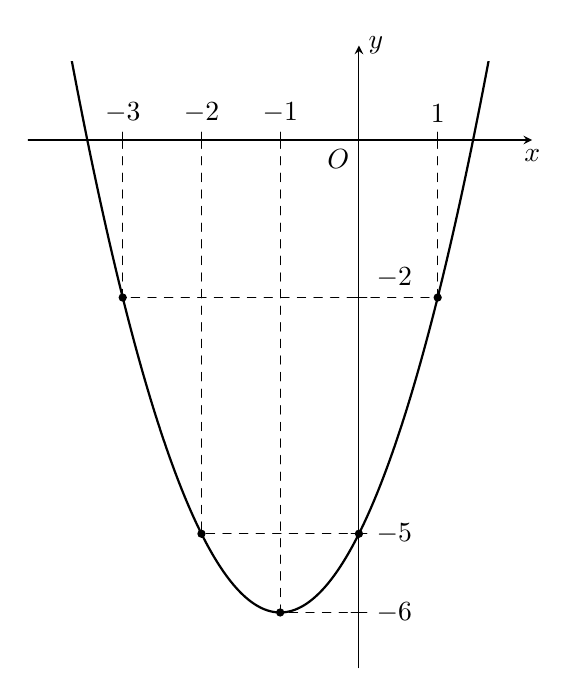
\begin{tikzpicture}[scale=1, line join=round, line cap=round, >=stealth]
			\tikzset{every node/.style={scale=1}}
			\def\xmin{-4}\def\xmax{2}\def\ymin{-6.5}\def\ymax{1}
			\draw[->] (\xmin-0.2,0)--(\xmax+0.2,0) node[below] {$x$};
			\draw[->] (0,\ymin-0.2)--(0,\ymax+0.2) node[right] {$y$};
			\draw (0,0) node [below left] {$O$};
			\foreach \x in {-3,-2,-1,1}\draw (\x,-0.1)--(\x,0.1) node [above] {$\x$};
			\foreach \y in {-5,-6}\draw (-0.1,\y)--(0.1,\y) node [right] {$\y$};
			\foreach \y in {-2}\draw (-0.1,\y)--(0.1,\y) node [above right] {$\y$};
			\clip (\xmin,\ymin) rectangle (\xmax,\ymax);
			\draw[thick,smooth,samples=200,domain=\xmin:\xmax] plot (\x,{1*((\x)^2)+2*\x+-5});
			\draw[dashed] (-3,0)--(-3,-2)--(0,-2);\fill (-3,-2) circle (1.5pt);
			\draw[dashed] (-2,0)--(-2,-5)--(0,-5);\fill (-2,-5) circle (1.5pt);
			\draw[dashed] (-1,0)--(-1,-6)--(0,-6);\fill (-1,-6) circle (1.5pt);
			\draw[dashed] (1,0)--(1,-2)--(0,-2);\fill (1,-2) circle (1.5pt);\fill (0,-5) circle (1.5pt);
		\end{tikzpicture}
	}
}
\end{bt}
\begin{bt}%[Dự án đề kiểm tra GHKI NH22-23- Nguyễn Sĩ Đạt]%[0T3B2-2]%Câu 7:
Xác định các hệ số $a$ và $b$ của hàm số bậc hai $y=ax^2+bx-10$. Biết đồ thị hàm số đi qua điểm $A(2; 14)$ và có trục đối xứng $x=-2$.
\loigiai{
	Đồ thị hàm số đi qua điểm $A(2; 14)$ suy ra $4a+2b=24$.\\
	Đồ thị hàm số có trục đối xứng $x=-2$ suy ra $-\dfrac{b}{2a}=-2\Leftrightarrow 4a-b=0$.\\
	Ta có hệ phương trình $\heva{&4a+2b=24\\&4a-b=0}\Leftrightarrow \heva{&a=2\\&b=8.}$
}
\end{bt}
